% Theorie: Physikalische Grundlagen von Versuch/Messverfahren, Gleichungen ohne Herleitung knapp erklären
\section{Theorie}
\label{sec:theorie}

\begin{figure}[H]
	\centering
	\includegraphics[width=0.5\linewidth]{content/grafik/formen.jpg}
	\caption{}
	\label{fig:formen}
\end{figure}

\subsection{Funktionsweise}

\begin{figure}[H]
	\centering
	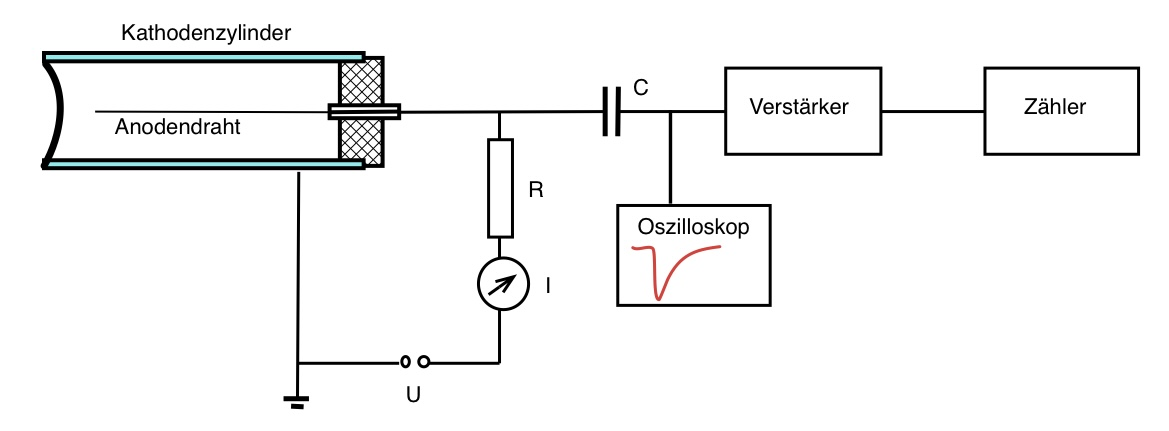
\includegraphics[width=0.9\linewidth]{content/grafik/diagramm.jpg}
	\caption{}
	\label{fig:diagramm}
\end{figure}

\subsection{Funktionsbereiche}

\subsubsection{Charakteristische Kennlinie}

\begin{figure}[H]
	\centering
	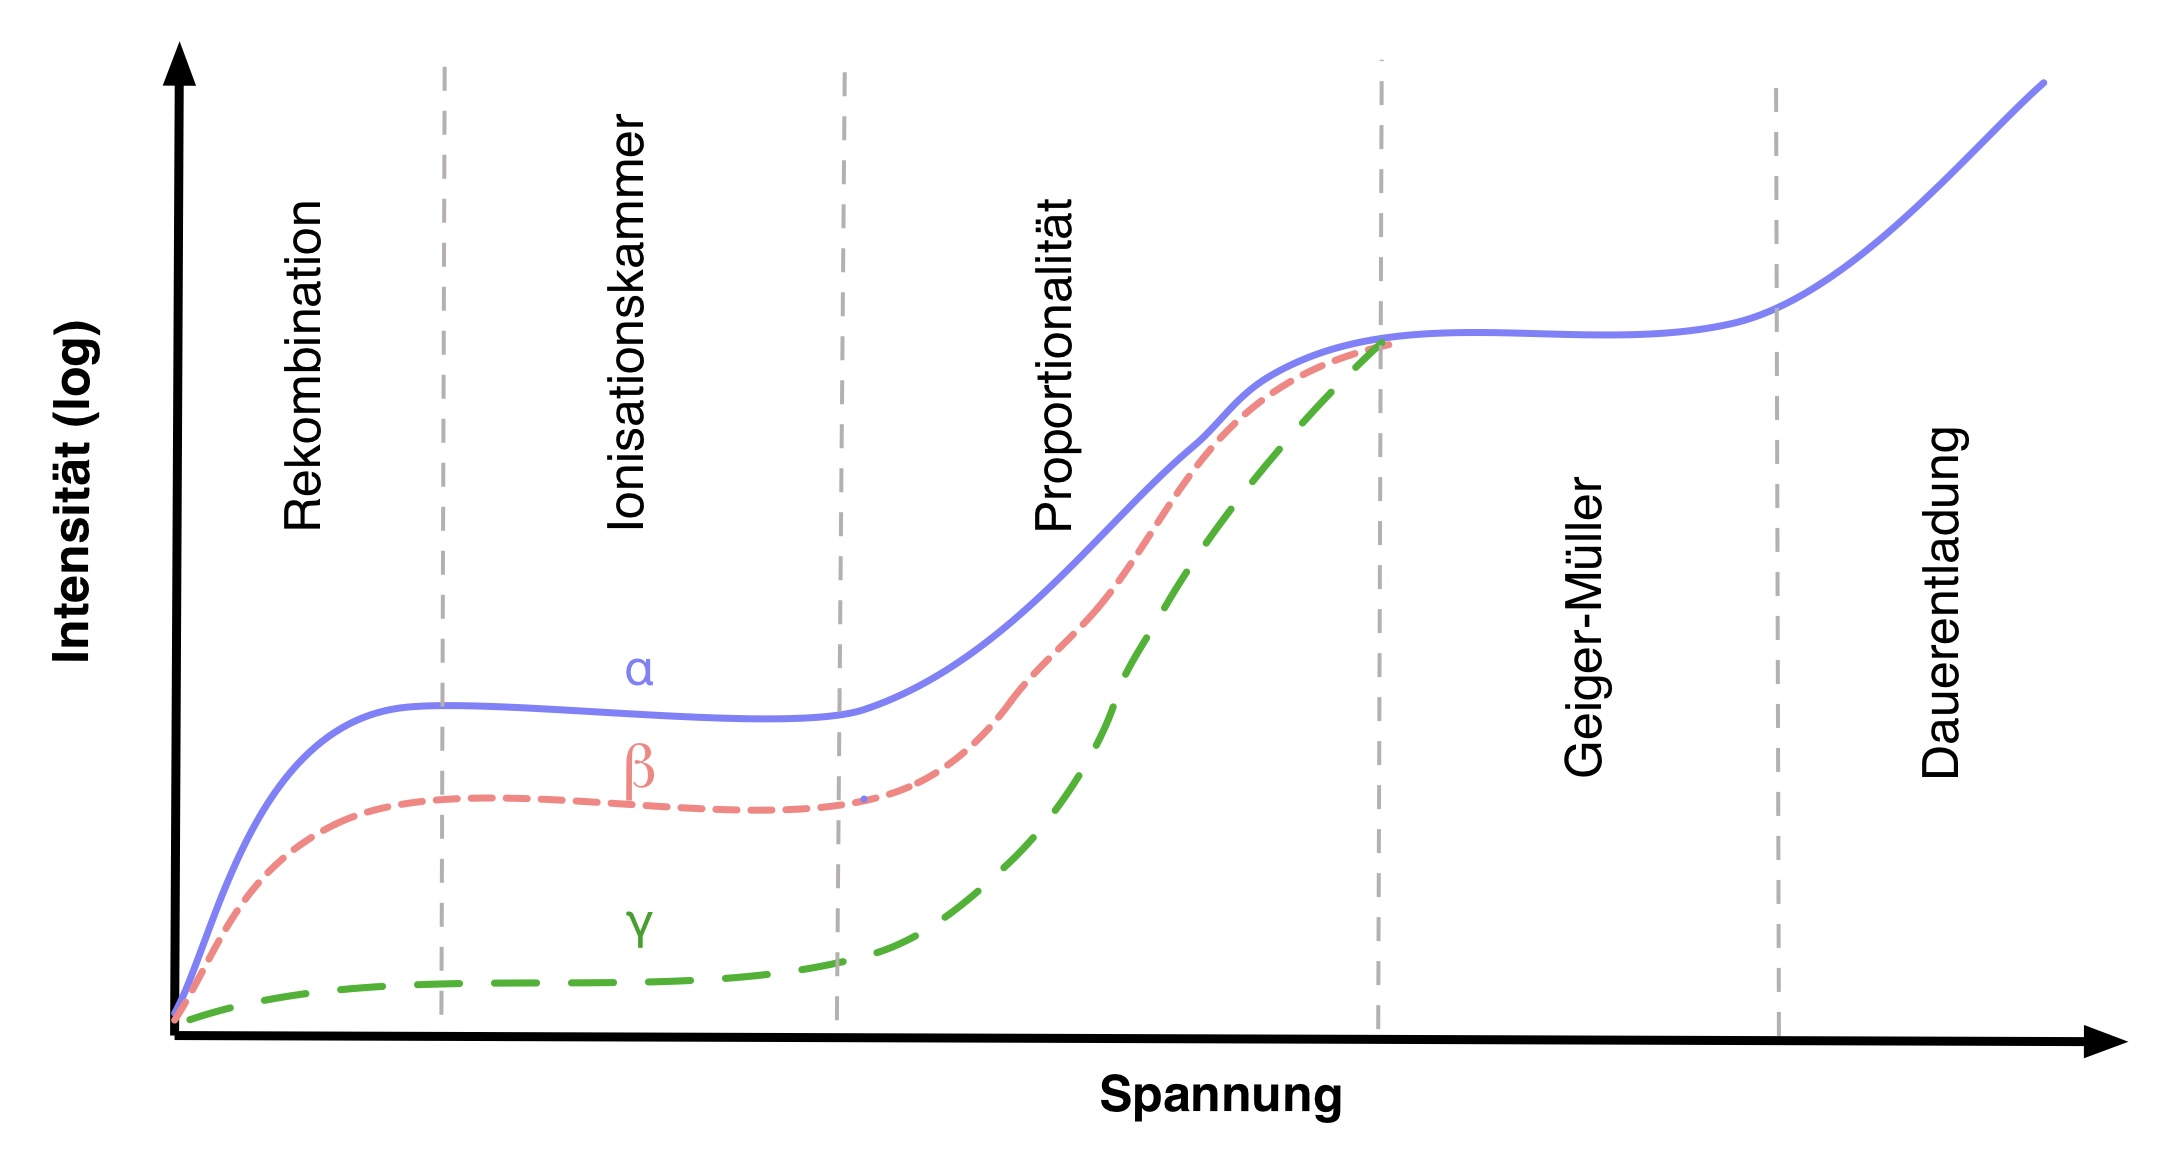
\includegraphics[width=0.9\linewidth]{content/grafik/kurve.jpg}
	\caption{}
	\label{fig:kurve}
\end{figure}

\paragraph{Rekombination}

\paragraph{Ionisationskammer}

\paragraph{Proportionalität}

\paragraph{Geiger-Müller}

\paragraph{Dauerentladung}

\subsubsection{Tot- und Erholungszeit}

\subsubsection{Güte des Plateaus}

\subsection{Statistik}

\begin{figure}[H]
	\centering
	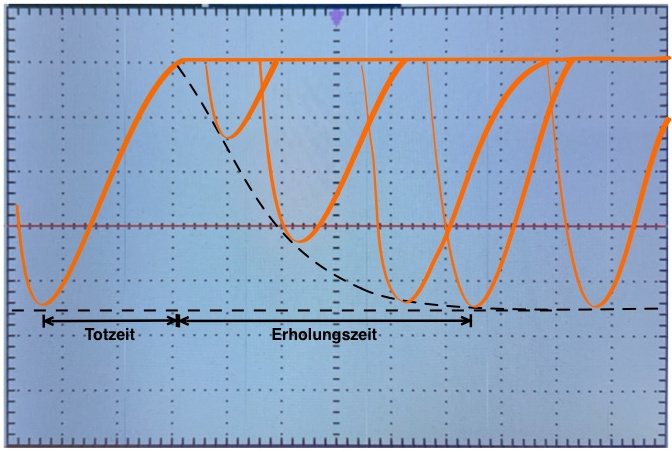
\includegraphics[width=0.5\linewidth]{content/grafik/zeit_soll.jpg}
	\caption{}
	\label{fig:zeit_soll}
\end{figure}

